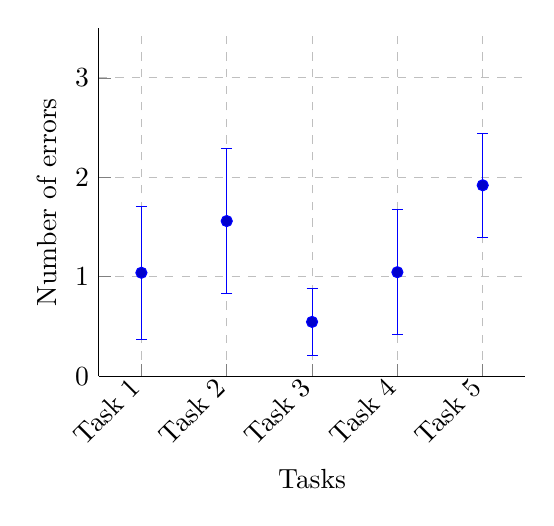
\begin{tikzpicture}[scale=1.0],
\centering
\begin{axis}[
height=6cm,
width=7cm,  
  xlabel={Tasks},
  ylabel={Number of errors}, 
  ymax=3.5,
  ymin=0,
  xmin=0.5,
  xmax=5.5,
  axis y line*=left,
  axis x line*=bottom,
  xticklabels={Task 1,Task 2,Task 3,Task 4,Task 5},
  xtick={1,...,5},
  ytick={0,1,...,20},
  ymajorgrids=true,
  xmajorgrids=true,
  grid style=dashed,
  x tick label style={rotate=45,anchor=east}]
\addplot+[only marks][error bars/.cd,y dir=both, y explicit]
coordinates {
(1,1.04) +- (0.668,0.668)
(2,1.56) +- (0.728,0.728)
(3,0.5455) +- (0.3365,0.3365)
(4,1.0455) +- (0.6283,0.6283)
(5,1.92) +- (0.5215,0.5215)
};
\addplot[dashed] coordinates {(0,0) (5.5,0)};
\end{axis}
\end{tikzpicture}%